\setchapterpreamble[u]{\margintoc}
\chapter{Summary and Outlook}

\section{Summary}
\label{sec:summary}

This work presented two oscillation measurements of atmospheric neutrinos using the DeepCore sub-array of the IceCube Neutrino Observatory.
Both measurements were based on a newly developed data sample of \num{21914} highly pure track-like events in the energy range between \SI{5}{\giga\electronvolt} and \SI{150}{\giga\electronvolt}.
The selection process for these events was described in \refch{data-sample} and consisted of several filtering steps in which background due to detector noise and atmospheric muons was removed.
At the final filter level, the contribution of muon background was reduced to $\sim2\%$, the noise background was entirely negligible and the sample consisted almost entirely of neutrino interactions.
The zenith angle of each event was reconstructed using a modified chi-square fit to the hit times of the observed light under the simplified assumption that they are well described by the Cherenkov light cone of a minimally ionizing muon.
This method required a cleaning step prior to the reconstruction that removes hits from photons that are likely to have undergone a significant amount of scattering.
Because the zenith reconstruction requires that at least five hits remain after the cleaning procedure, only a subset of all events could be reconstructed this way.
However, the stringent hit selection also resulted in a sample of high-quality events.

The energy was estimated with a likelihood that takes into account whether or not a sensor in the array has observed light.

Several quantities produced by the reconstruction algorithms, such as the length of the reconstructed track and the goodness-of-fit, were used as input variables for a Boosted Decision Tree (BDT) that calculates a particle ID (PID) score that estimates the probability of an event to have originated from a charged-current muon neutrino interaction.
Data and simulated pseudo-data were binned in zenith angle, energy, and PID.
The best-fit neutrino oscillation parameters were then fit by weighting the simulated events to match the histograms of the observed data as closely as possible.

\subsection{Three-Flavor Oscillation Measurement}
\label{sec:summary-three-flavor}

The first data analysis shown in this work was a measurement of the atmospheric mixing angle and mass splitting in the three-flavor neutrino oscillation model assuming normal mass ordering.
This measurement is complementary to oscillation analyses of accelerator neutrinos and constitutes the most precise measurement using atmospheric neutrinos to date.
The result,
\begin{align*}
    \sin^2\theta_{23} &= 0.507_{-0.053}^{+0.050}\\
    \Delta m^2_{32} &= 2.42_{-0.75}^{+0.77} \times10^{-3}\;\mathrm{eV}^2,
\end{align*}
is consistent with previous DeepCore measurements and current global fits.

\subsection{Sterile Neutrino Search}
\label{sec:summary-sterile-osc}

The second measurement presented in this work was the search for eV-scale sterile neutrinos.
The search was performed under the "3+1" model, where the PMNS matrix is extended by an additional row and column to accomodate the mixing of a fourth neutrino mass eigenstate.
The measurement used the same data sample as the three-flavor fit and the same likelihood function calculated in an identical binning.
The major technical difference between the analyses was that the neutrino oscillation calculation for the sterile neutrino model was done using a customized version of the \textsc{nuSQuIDS} package.
This allowed to efficiently calculate flavor transition probabilities in the presence of a heavy fourth mass eigenstate that produces a very fast oscillation pattern.
The customizations that were developed specifically for this work were the addition of low-pass filters that can analytically produce oscillation probabilities where the contributions due to that heaviest mass eigenstate are averaged out.
Another major technical development that separates the sterile neutrino analysis from the three-flavor fit is the introduction of a novel method of incorporating uncertainties in the detector response in a way that is fully decoupled from neutrino oscillation probabilities.

%\subsubsection{Result}
The analysis constrained the $|U_{\mu4}|$ and $|U_{\tau4}|$ elements of the extended PMNS matrix to\todo{extract precise numbers}
\begin{equation}
    \begin{aligned}
        \abs{U_{\mu4}}^2 &< X \\
        \abs{U_{\tau4}}^2 &< Y \\
    \end{aligned}
\end{equation}
at 90\% C.L. while marginalizing over the CP violating phase $\delta_{24}$. This result is valid for both normal ordering and inverted ordering due to the approximate degeneracy between the mass ordering and the sign of $\cos(\delta_{24})$. The confidence limits were calculated using Wilks' theorem assuming two degrees of freedom. Spot-checks of the likelihood distributions showed that these limits err on the conservative side. More stringent limits could be obtained by correcting the critical values of the likelihood according to Feldman and Cousins\cite{Feldman_1998}. However, the computational expense was estimated to be too high and the conservative limits sufficient for the purposes of this work. This result is a substantial improvement over the previous DeepCore result and provides the most stringent limit on $\abs{U_{\tau4}}^2$ to date. The constraint on $\abs{U_{\mu4}}^2$ is competitive with other experiments and has the potential to further increase the tension between appearance and disappearance datasets in global fits of the 3+1 sterile neutrino model described in \refsec{global-anomalies}.

\section{Outlook}

The measurement presented in this thesis only used the fraction of the available DeepCore data that could be reconstructed with established reconstruction methods that are optimized for robustness.
The purpose of this analysis was not to achieve the highest possible sensitivity, but to verify the integrity of the newly developed methods of data selection and of treating uncertainties in the detector properties.
Once the tools that were developed for this analysis are combined with more capable reconstruction methods, this new data sample will provide constraints on oscillation parameters that are more stringent than those of any other atmospheric neutrino oscillation measurement and rival the precision of the most recent accelerator experiments.

\subsection{Reconstruction Improvements}
A substantial increase in the sensitivity of both analyses could be achieved by using the table-based reconstruction method described in \cite{lowen-reco-paper}.
This algorithm can provide an estimate for the energy and zenith angle for nearly all events passing the Level 5 event filter described in \refsec{data-processing} and has a much higher resolution than the reconstruction method used in this analysis, substantially increasing the statistical power of the analysis.
The projected sensitivity that could be achieved with this method is shown in \reffig{retro-sensitivity}.\todo{Compare SANTA sensitivity, add retro sensitivity} With the increased statistical power and resolution also comes a larger burden to accurately model the properties of the neutrino flux, particle interactions and detector characteristics.\todo{Should we add a plot of our actual result?}The work to bring data and simulation into agreement for the higher statistics sample is still ongoing at the time of writing this thesis.
\begin{figure}
    \centering
    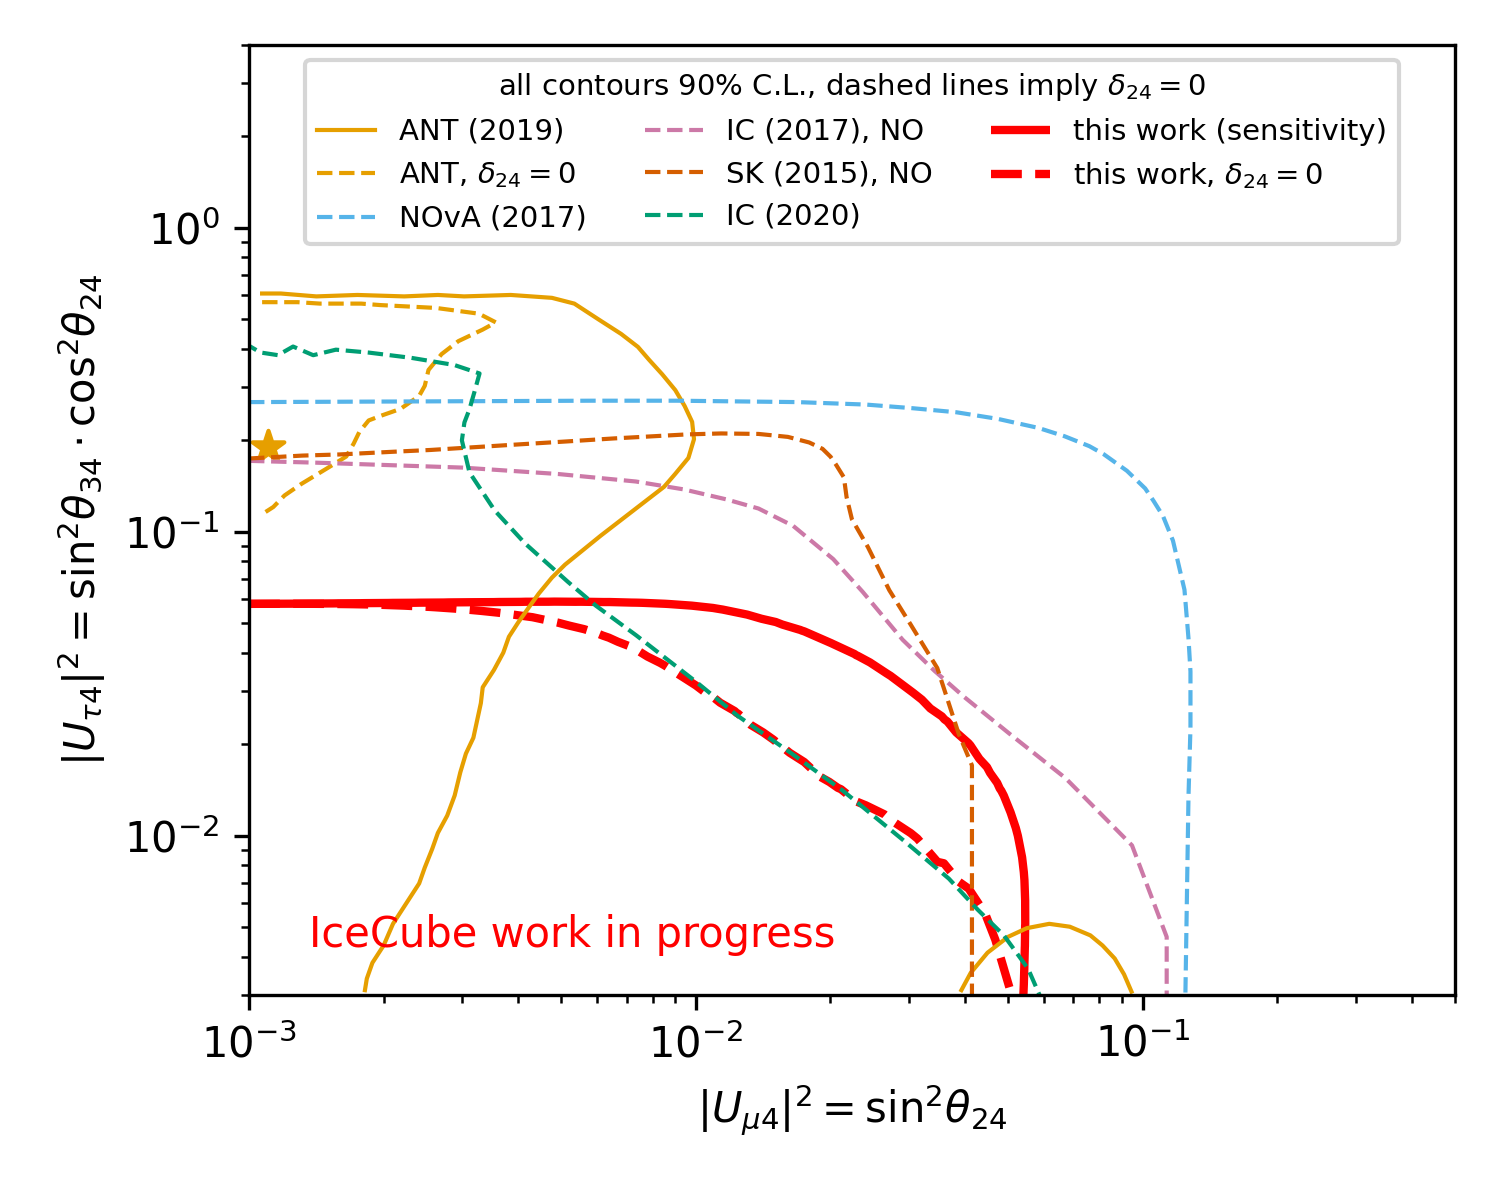
\includegraphics[width=0.9\linewidth]{figures/summary/Sterile_mixing_sensitivity_90pct_retro.png}
    \caption{Projected sensitivity of the sterile neutrino search when using the table-based reconstruction method.\label{fig:retro-sensitivity}}
\end{figure}

\subsection{Ice model}
The major distinction of the IceCube Neutrino Observatory compared to most other neutrino detectors is that the detection medium is the naturally occurring ice at the South Pole, rather than an artificially produced material.
The ice consists of many layers with different optical qualities that are the result of varying snow depositions over the last \num{100000} years.
Understanding the precise properties of the ice at every position in the detector requires complex calibration procedures that are beyond the scope of this work.
Recently, calibration efforts within IceCube have led to a new ice model that takes into account the birefringent scattering of light at the boundary of ice crystals\sidecite{tc-2022-174}.
The birefringence bends light rays into the direction of the flow of the glacier, which affects the zenith angle reconstruction for events in DeepCore in particular.
Future iterations of DeepCore oscillation studies are expected to include this new ice model in order to achieve a better agreement between data and simulation.

\subsection{Treatment of systematic uncertainties}
\subsubsection{Detector uncertainties}
In order to perform the sterile oscillation search, a novel method of interpolating between off-nominal MC sets has been developed that allows to weight individual events based on changes in the detector response.
The need for this development arose as the preceding uncertainty treatment showed artificial dependencies on the values of physics parameters.
In the three-flavor analysis, this problem was addressed by interpolating the gradients of the bin counts with respect to detector parameters on a grid in the mass splitting parameter $\Delta m^2_{31}$ as described in \refsec{hypersurfaces}.
For the sterile analysis, however, the dimensionality of such a grid made this approach unfeasible.
The newly developed method, described in \refsec{ultrasurfaces}, completely decouples the detector response from oscillation parameters and thereby eliminates the need for any interpolation.
This property makes this approach universally applicable to any oscillation study probing arbitrarily complex oscillation phenomena.
In addition, the method is compatible with unbinned likelihood functions in future analyses, unlike previous methods\sidecite{multisim} that are inherently binned.
This new method of calculating event-wise weights based on posterior estimates will be expanded upon and has the potential to become the new standard treatment for detector uncertainties for neutrino telescopes.

\subsubsection{Atmospheric flux}
The treatment of atmospheric neutrino flux uncertainties used in this work is based on the Barr blocks method that was published in 2006\cite{Barr2006}.
Since then, new methods of modeling variations of the atmospheric flux have been developed that decrease the overall relative uncertainty by up to 40\% and also provide a data-driven parametrization of the flux variations\sidecite{Fedynitch_2022}.
Incorporating these developments into the oscillation data analysis has the potential to improve the agreement between data and simulation and to increase the sensitivity.

\subsection{IceCube Upgrade}
The IceCube Collaboration will deploy seven strings of densely spaced optical sensors within the DeepCore fiducial volume in the near future that will form the \emph{IceCube Upgrade} \sidecite{icecube_upgrade}.
The Upgrade will not only be instrumented more densely than the existing DeepCore array, but will also contain new types of optical sensors that contain multiple PMTs.
This will increase the total photocathode density and add the ability to differentiate the arrival direction of light on each sensor.
The new array is expected to lower the energy threshold for the detection of atmospheric neutrinos to $\sim\SI{1}{\giga\electronvolt}$.
The Upgrade strings will also incorporate several calibration devices that will further improve the understanding of the ice and detector properties.
The sensitivity of the Upgrade array to neutrino oscillation parameters is expected to greatly improve over that of DeepCore as shown in \reffig{upgrade-sensitivity} for the atmospheric mass splitting and mixing angle.
\begin{figure}
    \centering
    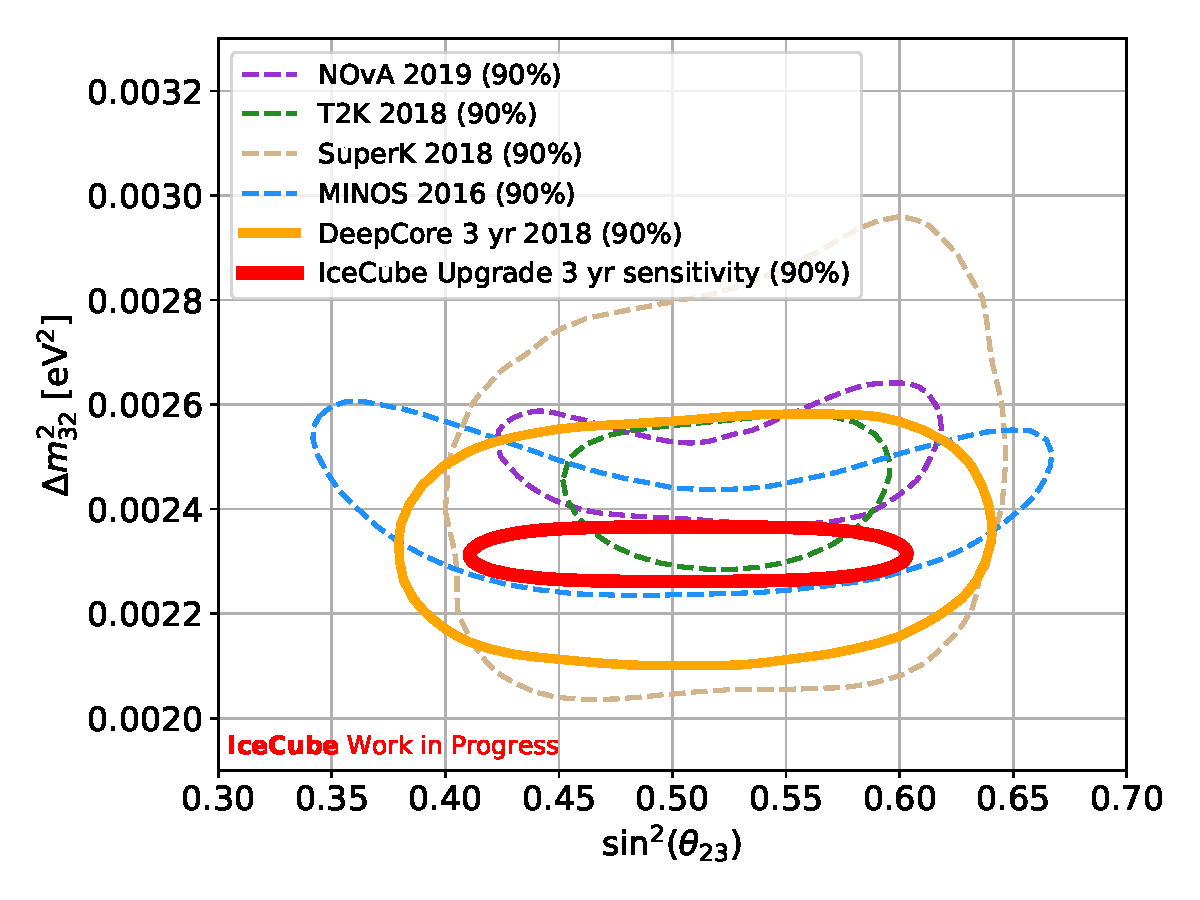
\includegraphics[width=0.7\linewidth]{figures/summary/June26_Upgrade_NuMu_Disappearance_Sensitivity.pdf}
    \caption{Expected sensitivity to the atmospheric neutrino oscillation parameters with three years of Upgrade data compared to recent results from DeepCore and other experiments. Figure taken from \cite{icecube_upgrade}.\label{fig:upgrade-sensitivity}}
\end{figure}


\chapter{Conclusion}

This thesis presented the first results obtained using a newly developed eight-year data sample of neutrinos produced in the atmosphere of the Earth, as detected by the IceCube DeepCore detector.
The sample is the result of a collaborative effort to improve the detector calibration\todo{should I mention calibration or not?} and selection process to achieve better agreement between data and simulation.
The events used for the measurement were reconstructed using a simple and fast geometric algorithm that reconstructs the direction for very clean, track-like events as well as an energy reconstruction based on a simple hit/no-hit likelihood.
With this sample of events, the analysis was able to achieve a good fit to the data and produce a measurement of the standard atmospheric neutrino oscillation parameters $\theta_{23}$ and $\Delta m^2_{32}$, as well as constraints on sterile neutrino mixing that are the best in this class of experiments.

The analysis also led to important developments of analysis tools and techniques that are directly applicable to studies with higher statistics and improved reconstruction methods.
These include a method of interpolating between different Monte Carlo sets in a way that is decoupled from neutrino oscillation effects, as well as several filtering techniques to efficiently calculate neutrino oscillation probabilities in the presence of heavy neutrino states.

The search for sterile neutrinos, which are a potential byproduct of the process that generates neutrino masses and might explain the different mass scale of neutrinos with respect to other SM particles, was performed by probing the $\nu_\mu$ disappearance probability under the assumption of the minimal "3+1" model with one additional mass splitting of $\order{\SI{1}{\electronvolt\squared}}$.
The choice of mass splitting was based on experimental anomalies found in accelerator experiments and measurements of the neutrino flux produced in radioactive decay.
The null-result of the search further increases the tension between the anomalies observed in the $\nu_e$ appearance channel probed in LSND and MiniBooNE and the constraints from $\nu_e$ and $\nu_\mu$ disappearance datasets.
Given that this tension already approached the $5\sigma$ threshold in global fits, it is unlikely that the simple "3+1" model of sterile neutrino oscillation can explain the anomalies that initially motivated the measurement.
The data selection and analysis methods developed during this work will enable future DeepCore measurements with greatly increased statistical power to probe neutrino oscillations for signals of a rich landscape of other possible phenomena beyond the Standard Model.
